\documentclass{article}
\usepackage[utf8]{inputenc}

\usepackage{amsmath}
\usepackage{hyperref}
\usepackage{array} % Import array package
\usepackage[letterpaper, portrait, margin=1in]{geometry}

\title{ECE120 Final Review - Cramming Carnival}
\author{Author: Members of HKN}
\date{Fall 2024}

\newcommand{\dd}[1]{\mathrm{d}#1}

\usepackage[makeroom]{cancel}
\usepackage[letterpaper, portrait, margin=1in]{geometry}
\usepackage{graphicx}
\usepackage{float}
\usepackage{enumitem}
\usepackage{graphicx}
\usepackage{multicol}

\pagenumbering{arabic}

\begin{document}

\maketitle

\section{Bitwise Bonanza}
\begin{enumerate}[label=(\alph*)]
    \item \textbf{Twos Complement Sign Extension}: Given the binary numbers in two’s complement, give the respective value as a 8-bit two’s complement representation (If given a 5-bit number, write the same value with 8-bits).
    \begin{enumerate}[label=(\roman*)]
        \item 010100
        \item 1010100
        \item 0001010
        \item 0100011
        \item 111000
        \item 10
        \item 00
        \item 01
        \item 1
    \end{enumerate}
    \item \textbf{Converting to Hexadecimal Notation}: Given the binary number below, convert to hexadecimal (Sign extend if necessary).
    \begin{enumerate}[label=(\roman*)]
        \item 1010100111010000
        \item 0101001111000001
        \item 1111011110001010
        \item 0100001110100101
    \end{enumerate}
    \item \textbf{Converting From Unsigned Representation}: Given the 5-bit \underline{unsigned} binary string, what is its decimal equivalent?
    \begin{enumerate}[label=(\roman*)]
        \item 10101
        \item 01010
        \item 11110
        \item 11011
    \end{enumerate}
    \item \textbf{Converting from IEEE 754 32-bit Floating Point}: Given the IEEE 754 32-bit Floating Point, what is its decimal equivalent?
    \begin{enumerate}[label=(\roman*)]
        \item 1 10000000 00010000000000000000000
        \item 0 01111111 10010000000000000000000
        \item 1 10000011 11000100000000000000000
    \end{enumerate}
    \newpage
    \item \textbf{Converting from Hexadecimal Notation}: Given the hexadecimal notation below, what is the binary representation?
    \begin{enumerate}[label=(\roman*)]
        \item 109F
        \item 74BC
        \item E235
        \item 86AD
    \end{enumerate}
    \item \textbf{Representation Integer Range}: What is the minimum number of bits needed to represent the values (which are in decimal) below?
    \begin{enumerate}[label=(\roman*)]
        \item 343
        \item 1709
        \item -123
        \item -1
        \item 0
    \end{enumerate}
    \item \textbf{Representing a Number Using Two's Complement Representation}: Give the 6-bit two's complement representation of the following decimal values.
    \begin{enumerate}[label=(\roman*)]
        \item -9
        \item -4
        \item 5
        \item 7
        \item -16
    \end{enumerate}
    \item \textbf{Converting to IEEE 754 32-bit Floating Point}: Enter the IEEE 754 32-bit floating point representation of each of the following decimal numbers.
    \begin{enumerate}[label=(\roman*)]
        \item $6 \frac{15}{16}$
        \item $4 \frac{1}{8}$
        \item $7 \frac{3}{4}$
    \end{enumerate}
    \item \textbf{Two's Complement Subtraction}: These numbers are in two’s complement representation.  Subtract the numbers.
    \begin{enumerate}[label=(\roman*)]
        \item 101001 - 111111
        \item 001101 - 001010
        \item 110010 - 110110
        \item 111100 - 000110
    \end{enumerate}
    \item \textbf{Two's Complement Addition Overflow}: For the following binary values, which of them have an overflow in 2’s complement?
    \begin{enumerate}[label=(\roman*)]
        \item 110001 + 100011
        \item 100100 + 001010
        \item 110010 + 111111
    \end{enumerate}
\end{enumerate}
\newpage
\section{Thrilling Toggles and Terrific Truth Tables}
\begin{enumerate}[label=(\alph*)]
    \item
        \textbf{D Flip-Flop Timing Diagram}: Given this image below of a timing diagram for a positive edge-triggered D flip-flop, sketch the values for Q at each time.
        \newline
        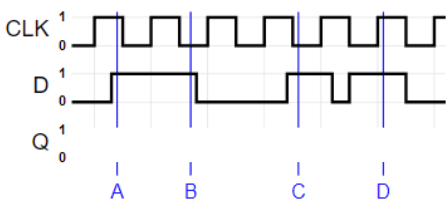
\includegraphics[width=15cm,height=6cm]{figures/DFlipFlop.png}
    \item 
        \textbf{CMOS Gate Truth Table (3 Variables)}: For the CMOS gate shown below, enter in the truth table output.
        \begin{multicols}{2}
        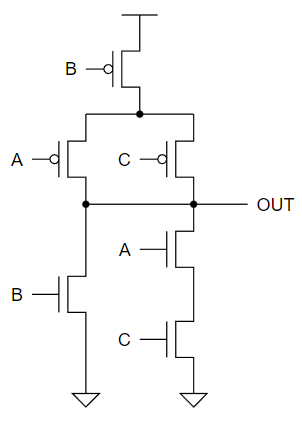
\includegraphics[width=7cm]{figures/CMOS.png}
        \columnbreak
        \begin{center}
        \scalebox{1.8} {
        \begin{tabular}{||c c c c||}
         \hline
         A & B & C & Out \\ [0.5ex] 
         \hline\hline
         0 & 0 & 0 &      \\
         \hline
         0 & 0 & 1 &  \\
         \hline
         0 & 1 & 0 &  \\
         \hline
         0 & 1 & 1 &  \\
         \hline
         1 & 0 & 0 &  \\ [1ex] 
         \hline
         1 & 0 & 1 &  \\ [1ex] 
         \hline
         1 & 1 & 0 &  \\ [1ex] 
         \hline
         1 & 1 & 1 &  \\ [1ex] 
         \hline
        \end{tabular}
        }
        \end{center}
        \end{multicols}
    \newpage
    \item
        \textbf{Boolean Expression to Truth Table}: Fill in the truth table given by the functions below.
        \begin{multicols}{2}
        \begin{enumerate}[label=(\roman*),nolistsep]
          \item F(A,B,C,D) = (A+B'+C)’D’
          \item G(A,B,C,D) = (A+B’)(CD+A)’ 
          \item H(A,B,C,D) = (CB)+A’D’B+B’CD
          \item I(A,B,C,D) = ACD+AB+(BC)’
        \end{enumerate}
        \columnbreak
        \begin{center}
        \scalebox{1.2} {
            \begin{tabular}{|c|c|c|c||c|c|c|c|}
            \hline
            \multicolumn{4}{|c||}{Inputs} & \multicolumn{4}{|c|}{Outputs} \\
            \hline
            A & B & C & D & F & G & H & I \\
            \hline
            0 & 0 & 0 & 0 & & & & \\
            0 & 0 & 0 & 1 & & & & \\
            0 & 0 & 1 & 0 & & & & \\
            0 & 0 & 1 & 1 & & & & \\
            0 & 1 & 0 & 0 & & & & \\
            0 & 1 & 0 & 1 & & & & \\
            0 & 1 & 1 & 0 & & & & \\
            0 & 1 & 1 & 1 & & & & \\
            1 & 0 & 0 & 0 & & & & \\
            1 & 0 & 0 & 1 & & & & \\
            1 & 0 & 1 & 0 & & & & \\
            1 & 0 & 1 & 1 & & & & \\
            1 & 1 & 0 & 0 & & & & \\
            1 & 1 & 0 & 1 & & & & \\
            1 & 1 & 1 & 0 & & & & \\
            1 & 1 & 1 & 1 & & & & \\
            \hline
            \end{tabular}
        }
        \end{center}
        \end{multicols}
    \item
        \textbf{Truth Table to SOP and POS}: Using the truth table below, express outputs F1 and F2 as a minimal sum of products (SOP) and a minimal product of sums (POS).
        \begin{multicols}{2}
        \begin{center}
        \scalebox{1.2} {
            \begin{tabular}{|c|c|c|c||c|c|}
            \hline
            A & B & C & D & F1 & F2 \\
            \hline
            0 & 0 & 0 & 0 & 1 & 1 \\
            0 & 0 & 0 & 1 & 1 & 0 \\
            0 & 0 & 1 & 0 & 0 & 0 \\
            0 & 0 & 1 & 1 & x & 1 \\
            0 & 1 & 0 & 0 & 0 & 1 \\
            0 & 1 & 0 & 1 & 0 & 0 \\
            0 & 1 & 1 & 0 & 1 & 1 \\
            0 & 1 & 1 & 1 & x & x \\
            1 & 0 & 0 & 0 & 1 & 0 \\
            1 & 0 & 0 & 1 & 0 & 0 \\
            1 & 0 & 1 & 0 & 0 & 1 \\
            1 & 0 & 1 & 1 & 1 & 1 \\
            1 & 1 & 0 & 0 & 0 & x \\
            1 & 1 & 0 & 1 & 1 & 1 \\
            1 & 1 & 1 & 0 & 0 & 1 \\
            1 & 1 & 1 & 1 & x & 0 \\
            \hline
            \end{tabular}
        }
        \end{center}
        \columnbreak
        F1 (SOP) = 
        \newline
        \newline
        F1 (POS) = 
        \newline
        \newline
        F2 (SOP) = 
        \newline
        \newline
        F2 (POS) = 
        \newline
        \newline
        \end{multicols}
    \newpage
\end{enumerate}
\section{Multiplexer Mania}
    \textbf{Multiplexer to Boolean Formula}: Give the minimal SOP for F for the multiplexer below (express F in terms of the inputs).
    \newline
    \begin{multicols}{2}
    \begin{center}
    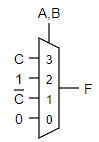
\includegraphics[width=3cm]{figures/Multiplexer.png}
    \end{center}
    \columnbreak
    \text{F(A,B,C) =}
    \end{multicols}
\section{Funky FSMs}
    \begin{enumerate}[label=(\alph*)]
        \item \textbf{FSM Design Application}: Given the FSM below:
        \begin{enumerate}[label=(\roman*),nolistsep,itemsep = 60pt]
            \item Find the K-Maps for S1+,S0+, and F.
            \item Give their minimal SOP Boolean logic expressions.
            \item Implement the FSM as D flip-flops and gates.
        \end{enumerate}
        \begin{multicols}{2}
        \begin{center}
        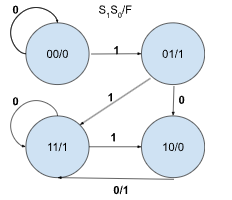
\includegraphics[width=6cm]{figures/FSMDesign.png}
        \end{center}
        \columnbreak
        \end{multicols}
        \newpage

        \item \textbf{FSM Counter}: Given the FSM below:
        \begin{enumerate}[label=(\roman*),nolistsep,itemsep = 60pt]
            \item Find the K-Maps for S2+,S1+, and S0+.
            \item Give their minimal SOP Boolean logic expressions.
        \end{enumerate}
        \begin{multicols}{2}
        \begin{center}
        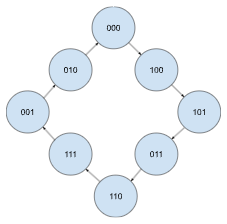
\includegraphics[width=6cm]{figures/FSMClock.png}
        \end{center}
        \columnbreak
        \end{multicols}

    \item \textbf{FSM Sequence Detector}: Generate an FSM that detects the sequence 001: 
    
    Input sequence M (starting from left to right):  100110100101  
    
    Output sequence R (Starting from left to right):  00010000010

    \begin{enumerate}[label=(\roman*),nolistsep,itemsep = 60pt]
        \item State declaration table
        \item The K-Maps for S1+,S0+, and F
        \item Give their minimal SOP Boolean logic expressions
    
    \end{enumerate}


\newpage
\section{Rambunctious RAM}
    \textbf{RAM Concepts}: Use the RAM Module Below to answer the questions:
    \newline
    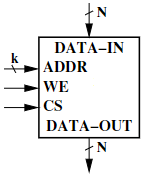
\includegraphics{figures/RAM.png}
    \begin{enumerate}[label=(\alph*),itemsep = 10pt]
        \item If there are k ADDR wires and N DATA-IN wires, what size memory does this chip store? (Hint: AxB)
        \item After entering the chip and before being input to a cell, what do the k wires enter?
        \item If given four 4x4 RAM blocks and any decoder possible, what sizes of RAM could be made?
        \item In a 16x8 RAM do the following tasks
        \begin{enumerate}[label=(\roman*),itemsep = 10pt]
            \item Write 0x12 into address 0x578A
            \item Write 0x72 into address 0xECEB
            \item Read from address 0x893F
        \end{enumerate}
    \end{enumerate}
\section{Legendary LC3}
    \begin{enumerate}[label=(\alph*)]
        \item \textbf{LC-3 bits to RTL}: For each of the following 16-bit sequences, give the RTL equivalent:
        \begin{enumerate}[label=(\roman*),itemsep = 10pt]
            \item 0001 1000 0100 0100
            \item 0101 0000 0011 1111
            \item 0000 1101 1111 1100 
            \item 0010 1000 0000 0111
            \item 1001 1010 0011 1111
        \end{enumerate}
        \newpage
        \item \textbf{LC-3 FSM Concepts (Von Neumann model)}: Answer the conceptual questions below:
        \begin{enumerate}[label=(\roman*),itemsep = 10pt]
            \item What are the first 3 FSM instructions the LC-3 executes with each line of code in memory?
            \item If the ALUK value is 00 what is the opcode of the line currently being performed?
            \item How many gates (that go to BUS) can be active at a time?
            \item Which opcodes set CC?
            \item In the von Neumann model, where is the program stored?
            \item How many steps are there at minimum in an instruction cycle?
        \end{enumerate}
        \item \textbf{LC-3 Programming}: Write the following functions in RTL (For each part, assume your first line starts at x3000 and all registers are x3000. Each part is independent of the others.)
        \begin{enumerate}[label=(\roman*),itemsep = 10pt]
            \item Given a value in x3005, set its 2’s complement in x3006
            \item Get an input from the keyboard and store it at x3030 (GETC = x20)
            \item Given two values in x3004 and x3005 store their sum in x3006
            \item Given two values in x3004 and x3005 store their product in x3006
            \item Using only register R1, and not accessing any other register, determine if the value stored in R2 is a power of 2 (you may also edit the value in R2)
        \end{enumerate}
        \item \textbf{String Programming}: After the following code executes, what will be printed to the console? Assume that the data in the table has already been loaded into memory when the code is run.
        \newline
        \newline
        .ORIG x3000
        \newline
        LD R0, STRING
        \newline
        PUTS
        \newline
        STRING
        \newline
        	.FILL 0x3047
        \newline
        .END
        \newline
        \begin{table}[h]
        \centering
        \begin{tabular}{|c|c|c|}
        \hline
        \textbf{Address} & \textbf{Data} & \textbf{ASCII Representation} \\\hline
        x3046 & x0021 & ‘!’ \\\hline
        x3047 & x0048 & ‘H’ \\\hline
        x3048 & x0069 & ‘i’ \\\hline
        x3049 & x0000 &     \\\hline
        x304A & x0074 & ‘t’ \\\hline
        x304B & x0068 & ‘h’ \\\hline
        x304C & x0065 & ‘e’ \\\hline
        x304D & x0072 & ‘r’ \\\hline
        x304E & x0065 & ‘e’ \\\hline
        x304F & x0021 & ‘!’ \\\hline
        x3050 & x0000 &     \\
        \hline
        \end{tabular}
        \end{table}
        \newline
        (i) How many memory locations will the following string use?
        \newline
        .STRINGZ “AMONG US”
        \newpage
        \item \textbf{Executing ALU Instructions}: The following sequence of instructions is executed with the initial register values shown below.
        \newline
        \newline
        x3000: 0001000001000011
        \newline
        x3001: 0101011011000001
        \newline
        x3002: 0101001000100000
        \newline
        R0: xA25B
        R1: x1B2A
        R2: x4875
        R3: x6227
        \newline
        \newline
        (i) Give the contents of the following registers after the instruction sequence above finishes executing. Convert your answers to hexadecimal.
        \item \textbf{LC3 Missing Instruction}
        \begin{enumerate}[label=(\roman*)]
            \item An LC-3 computer starts with the following register and memory contents. In addition, the word at address x3000, which is not shown, contains an instruction, one of ADD, AND, BR, LD, LDI, LDR, LEA, NOT, ST, STI, or STR. Note: The LEA instruction does not change the CC register (3rd edition behavior).
            \begin{table}[h]
            \centering
            \begin{tabular}{|c|c|c|}
            \hline
            \textbf{Registers} & \textbf{Memory} & \\
            \hline
            R0: x619F & & \\
            \hline
            R4: x48AA & & \\
            \hline
            R1: x4295 & x3001: x4333 & \\
            \hline
            R5: x49FC & x3002: x1BDC & \\
            \hline
            R2: x259D & & \\
            \hline
            R6: x54C2 & & \\
            \hline
            R3: x4000 & x4000: x2911 & \\
            \hline
            R7: xF914 & x4001: x68A8 & \\
            \hline
            PC: x3000 & & \\
            \hline
            CC: b001 & & \\
            \hline
            \end{tabular}
            \caption{Before: Registers and Memory}
            \label{tab:before}
            \end{table}
            \newline
            All other memory locations start with x0000. After the instruction at address x3000 is executed, the contents of registers and memory are:
            \begin{table}[h]
            \centering
            \begin{tabular}{|c|c|c|}
            \hline
            \textbf{Registers} & \textbf{Memory} & \\
            \hline
            R0: x619F & & \\
            \hline
            R4: x48AA & & \\
            \hline
            R1: x4295 & x3001: x4333 & \\
            \hline
            R5: x49FC & x3002: x1BDC & \\
            \hline
            R2: x259D & & \\
            \hline
            R6: x48B8 & & \\
            \hline
            R3: x4000 & x4000: x2911 & \\
            \hline
            R7: xF914 & x4001: x68A8 & \\
            \hline
            PC: x3001 & & \\
            \hline
            CC: b001 & & \\
            \hline
            \end{tabular}
            \caption{After: Registers and Memory}
            \label{tab:after}
            \end{table}
            \newline
            What value could be stored at address x3000? Give your answer in hexadecimal.
            \newline
            \newline
            x3000 = 
        \newpage
        \item An LC-3 computer starts with the following register and memory contents. In addition, the word at address x3000, which is not shown, contains an instruction, one of ADD, AND, BR, LD, LDI, LDR, LEA, NOT, ST, STI, or STR. Note: The LEA instruction does not change the CC register (3rd edition behavior).
            \begin{table}[h]
            \centering
            \begin{tabular}{|c|c|c|}
            \hline
            \textbf{Registers} & \textbf{Memory} & \\
            \hline
            R0: x619F & & \\
            \hline
            R4: x48AA & & \\
            \hline
            R1: x4295 & x3001: x4333 & \\
            \hline
            R5: x49FC & x3002: x1BDC & \\
            \hline
            R2: x259D & & \\
            \hline
            R6: x54C2 & & \\
            \hline
            R3: x4000 & x4000: x2911 & \\
            \hline
            R7: xF914 & x4001: x619F & \\
            \hline
            PC: x3000 & & \\
            \hline
            CC: b001 & & \\
            \hline
            \end{tabular}
            \caption{Before: Registers and Memory}
            \label{tab:before}
            \end{table}
            \newline
            All other memory locations start with x0000. After the instruction at address x3000 is executed, the contents of registers and memory are:
            \begin{table}[h]
            \centering
            \begin{tabular}{|c|c|c|}
            \hline
            \textbf{Registers} & \textbf{Memory} & \\
            \hline
            R0: x619F & & \\
            \hline
            R4: x48AA & & \\
            \hline
            R1: x4295 & x3001: x4333 & \\
            \hline
            R5: x49FC & x3002: x1BDC & \\
            \hline
            R2: x259D & & \\
            \hline
            R6: x48B8 & & \\
            \hline
            R3: x4000 & x4000: x2911 & \\
            \hline
            R7: xF914 & x4001: x68A8 & \\
            \hline
            PC: x3001 & & \\
            \hline
            CC: b001 & & \\
            \hline
            \end{tabular}
            \caption{After: Registers and Memory}
            \label{tab:after}
            \end{table}
            \newline
            What value could be stored at address x3000? Give your answer in hexadecimal.
            \newline
            \newline
            x3000 =
        \end{enumerate}
        \newpage
    \end{enumerate}
    \section{Fortuitous FSMs}
    Note: You may get different answers for this section as these problems are design heavy and are based on your understanding of the problem
    \begin{enumerate}[label=(\alph*), itemsep = 120pt]
        \item \textbf{Self Looping FSMs} In our daily lives, FSMs are used everywhere. Sometimes we do not realize it but almost everything around us is a FSM. One such example is a Sewage lift station that helps to manage wastewater generated by us. The lift station works by starting a pump that pumps out wastewater from the sludge tank when wastewater reaches the upper limit of the tank. The lift station will continue to pump out the wastewater till the water level is lower than the minimum water level in the tank. Given 2 signals \textbf{U for the upper limit (U=1 when water reaches upper limit)} and \textbf{L for the lower limit (L=0 when water level is lower than the lower limit)}, design the FSM for the lift station
        \begin{enumerate}[label=(\roman*), itemsep = 120pt]
            \item Draw the state transition diagram for this FSM. Your output should be the signal P, where P=1 indicates the pump should be running
            \item Create K-maps for next state and output of the FSM
            \item Write the next state expressions for the FSM
            \item Implement this FSM using gates, Combinational Logic Elements, Flip-Flops, RAMs etc
        \end{enumerate}
    \end{enumerate}
    \newpage

    \section{Liberating Loading}
    \begin{enumerate}[label=(\alph*), itemsep = 120pt]
        \item A memory address, pointing to the start of an array is stored at x30AD. Which load instruction type would you use to access the first array value? Write the single LC-3 assembly instruction to accomplish this when the PC is at x3090.
        \item What state numbers of the LC-3 FSM are used for a LDR instruction? Which of these states are unique only to LDR?
        \item Fill in the following table with the correct control signals on the LC-3 data path for the LDR Instruction. Note: This table doesn't have all the states for LDR.
        \vspace{0cm}
       
        \begin{table}[h]
            \centering
            \begin{tabular}{|>{\centering\arraybackslash}p{2.5cm}|>{\centering\arraybackslash}p{2.5cm}|>{\centering\arraybackslash}p{2.5cm}|>{\centering\arraybackslash}p{2.5cm}|}
            \hline
            \textbf{States} & \textbf{18} & \textbf{25} & \textbf{27} \\
            \hline
            LD.BEN & & & \\
            \hline
            LD.MAR & & & \\
            \hline
            LD.MDR & & & \\
            \hline
            LD.IR & & & \\
            \hline
            LD.PC & & & \\
            \hline
            LD.REG & & & \\
            \hline
            LD.CC & & & \\
            \hline
            GateMARMux & & & \\
            \hline
            GateMDR & & & \\
            \hline
            GateALU & & & \\
            \hline
            GatePC & & & \\
            \hline
            MARMUX & & & \\
            \hline
            PCMUX & & & \\
            \hline
            ADDR1MUX & & & \\
            \hline
            ADDR2MUX & & & \\
            \hline
            DRMUX & & & \\
            \hline
            SR1MUX & & & \\
            \hline
            ALUK & & & \\
            \hline
            MIO.EN & & & \\
            \hline
            R.W & & & \\
            \hline
            \end{tabular}
            \label{tab:modified}

        \end{table}
    \end{enumerate}
     \newpage

    \section{Manic Multiplying}
    You are going to complete a program that multiplies two numbers from memory together and saves the result back into memory. Below are the memory locations for the inputs and output. While you don't have to specify a .ORIG instruction for this problem, it is relevant that the program begins at x3000.
    \begin{table}[h]
        \centering
        \begin{tabular}{|c|c|c|}
        \hline
        \textbf{Meaning} & \textbf{Address} \\\hline
        Multiplicand 1 & x3FFE \\\hline
        Multiplicand 2 & x3FFF \\\hline
        Product & x4000 \\
        \hline
        \end{tabular}
        \end{table}
    \begin{enumerate}[label=(\alph*), itemsep = 140pt]
        \item Load Multiplicand 1 and Multiplicand 2 into R1 and R2, respectively. This will require 2 LC-3 instruction lines and 2 pre-processor instruction lines (ie .STRINGZ, .FILL, etc).
        \item Create a loop to multiply the multiplicands together and place the result in R3. You are allowed to modify R1 and R2 as needed.
        \item Store R3 into the product memory location. this will require 1 LC-3 instruction line and 1 pre-processor instruction line.

    \end{enumerate}
    \newpage
    
    \section{Disorienting Decoding}
    \begin{enumerate}[label=(\alph*), itemsep = 120pt]
        \item In the LC-3, if the IRD control signal is set to 1, what happens to the contents of the instruction register (IR) during the decoding process? Specifically, how are the bits IR[15:12] utilized?
        \item Given a situation where COND is set to 001, which represents checking for a positive condition code (P), and the instruction’s execution previously set the P flag to 1, what would be the value of BEN (branch enable)?
        \item Suppose the current instruction has an opcode of 1101 in IR[15:12], corresponding to a LEA instruction. If the J bits in the microinstruction are set to 011111, explain how the next state of the microsequencer is determined.
        \vspace{4cm}
        \begin{figure}[ht]
            \centering
            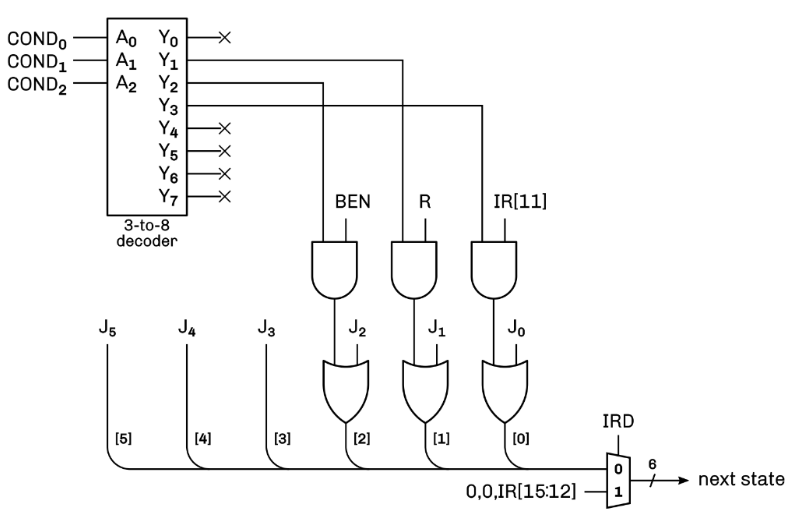
\includegraphics[width=10cm,height=4cm]{figures/microsequencer.png}
            \caption{LC-3 Microsequencer}
            \label{fig:optionalLabel}
            \end{figure}
        \newpage
    \end{enumerate}
    
    \section{Conspicuous Control Signals}
    \begin{enumerate}[label=(\alph*),itemsep = 120pt]
        \item Complete the following table by entering values (0, 1, or X) for the LC-3 microinstructions at ROM addresses 4 and 7
        
        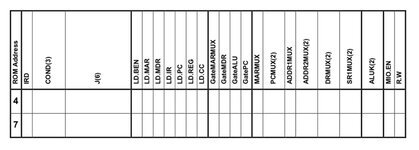
\includegraphics{figures/ControlSignals.jpg}
        \item If GateALU=1, what should the other Gate signals be?
        \newpage
    \end{enumerate}
    
    \section{Novel New Instructions}
    We want to implement the following instruction: \\
    PC $\longleftarrow$ PC + M[BaseR + PCOffset6] + 1 \\\\
    Note: the +1 is to accommodate state 18. \\
    Note 2: In the very rare case that you actually read the textbook, pretend Appendix C.6.3 did not exist.\\
    \begin{enumerate}[label=(\alph*),itemsep = 70pt]
        \item We know that LC-3 has one unused opcode, the opcode 1101. When this opcode is decoded, suppose that the LC-3 FSM enters state 48 (110000). How many FSM states will this instruction need? What will each state do? Assign them in the 48-55 range.
        \item How will each instruction transition to each other state? Draw a state diagram.
        \item Using K-maps or another method, write an expression for the next state transition that can be used after entering your first state and before entering state 18. (Hint: $S_5S_4S_3 = 110$, and memory ready is the signal $R$. you can work with the 4 bits $RS_2S_1S_0$)
        \item Using a similar table as in Problem 8, write down the control signals for each state.
        \item Trace through your instruction with the following instruction: \\
        1101 000 101 000111 \\
        Assume PC = x3001, R5 = x2000, and M[x2007] = x8EED. \\
        What is PC after the instruction completes and before the next execution of state 18?
    \end{enumerate}
    
    \newpage \section{Challenging Conundrums (Just For Fun)}
    Unless otherwise specified, you may use any registers you would like and store results in any register
    \begin{enumerate}[label=(\alph*), itemsep = 120pt]
        \item Using only three lines of code, set R0 = 0, R1 = 4, and R2 = -3
        \item Implement R1 NOR R2 in only 3 lines of code
        \item Implement R3 XOR R4 in only 5 lines of code
        \item Implement R5 OR R6 in only 4 lines of code
    \end{enumerate}
\end{document}